\section{Stability of the numerical method}
\subsection{Description}
\subsubsection{Principle}
In order to prove the stability of the temporal scheme, we can recall the following result concerning integration methods \cite{Geradin}: An integration scheme is said to be stable if there exists an integration step $h_0 > 0$ so that for any $h \in [0, h_0]$, a finite variation of the state vector at time $t^n$ induces only a non-increasing variation of the state vector $X^{n+1}$ calculated at a subsequent instant $t^{n+1}$.\\
In our case we will study the stability of the scheme with the temporal discretization presented in the previous section. We will focus our attention on the stability of the temporal scheme applied on only one element. If we can prove the stability on one element, the result extends to the others \cite{Belytschko}. \\
Therefore, if we define 2 initial states: a non-perturbed $X_0$  and a perturbed $X^\prime_0$ one. We can define the initial disturbance:
\begin{equation}
\delta X_0 = X^\prime_0 - X_0
\end{equation}
The state vector of the non-perturbed solution is defined in function of the amplification matrix $H$:
\begin{align}
X_{n+1} &= H X_n + g_{n+1} \\
&= H^2 X_{n-1} + Hg_n + g_{n+1} \\
&\vdots\\
&= H^{n+1}X_0 + \sum^{n+1}_{j=0} H^{n-j+1}g_j
\label{eq:nondist-tn1}
\end{align}
This formulation permits to express the state vector at a time $t_{n+1}$ in function of the amplification matrix and the initial solution $X_0$. The perturbed solution can be expressed in the same manner:
\begin{equation}
X^\prime_{n+1} = H^{n+1}X_0^\prime + \sum^{n+1}_{j=0} H^{n-j+1}g_j
\label{eq:dist-tn1}
\end{equation}
Therefore the effect of the disturbance can be expressed at the time $t_{n+1}$ by subtracting \ref{eq:dist-tn1} to \ref{eq:nondist-tn1}:
\begin{equation}
\delta X_{n+1} = H^{n+1} \delta X_0
\end{equation}
% How to obtain the eigenvalue problem
The resulting eigenvalue problem is defined by:
\begin{equation}
det(H-\lambda I) = 0
\end{equation}
We can define $\lambda_r, x_{(r)}$ the associated eigenvalues and eigenvectors of the amplification matrix.
The initial disturbance can be expressed as a combination of the eigenvectors:
\begin{equation}
\delta X_0 = \sum^{2N}_{s=1} a_s x_{(s)}
\label{eq:eig-dist}
\end{equation}
The recurrence relationship for the disturbance can be changed using \ref{eq:eig-dist} to obtain:
\begin{align}
\delta X_{n+1} &= H^{n+1} \sum^{2N}_{s=1} a_s x_{(s)} \\
&= \sum^{2N}_{s=1} a_s \lambda_s^{n+1} x_{(s)}
\end{align} 
Using this formulation we can observe that the disturbance will be amplified if the moduli of the eigenvalues of the amplification matrix are higher than $1$. In order to maintain the stability of a numerical scheme the spectral radius of the eigenvalues has to remain below $1$. \\
 
To apply this method to our PML scheme, described by the equations \ref{eq:newmark2} and \ref{eq:2Dpml-discrete-motion}, we have to construct the amplification matrix. We seek a system of equation such as:
\begin{equation}
 A(h) X_{n+1}  + B(h) X_{n} = 0  
\end{equation}
And the amplification matrix $H$ will be defined as:
\begin{equation}
 X_{n+1} = - A^{-1} B(h) X_{n} = H X_{n}  
\end{equation}
\subsubsection{Definitions of the stability criterion}
To obtain the proof of the stability of the integration scheme associated with the PML and to have some insights about its accuracy we have to define the different parameters that will be calculated and analysed. \\
First of all to prove the stability of the scheme we will calculate the eigenvalues of the amplification matrix. By representing them in the complex plane and by calculating the spectral radius we will conclude about the stability. In fact, only the spectral radius can lead to a conclusion about the stability of a scheme, but in the analysis of the results all moduli of all eigenvalues will be represented. This will allow us to see clearly the evolution of the different eigenvalues separately in function of the time step $h$.\\ 
The spectral radius is defined by:
\begin{equation}
\rho(H(h)) = \max_i |\lambda_i| 
\end{equation}
If the scheme is unconditionally stable the spectral radius over all the values of time step has to remain below the value $1$ and the representation of the eigenvalues in the complex space will remain within the unit circle. If the scheme is conditionally stable, we will be able to define the limit of stability, i.e. the time step for which the spectral radius is larger than $1$.\\
To be able to analyse the accuracy of the scheme, we will use two parameters: the numerical damping $\overline{\epsilon}$ and the relative periodicity error $\frac{\Delta T}{T}$. The numerical damping is a measure of the amplitude error and is defined for the time step $h$ and the eigenvalue $\lambda_i$ by: 
\begin{equation}
\overline{\epsilon} \omega h = -\frac{1}{2}\log(|\lambda_i|)
\end{equation}      
and the relative periodicity error by:
\begin{equation}
\frac{\Delta T}{T} = \frac{\omega_i}{\overline{\omega_i}} - 1
\end{equation}
\subsubsection{Material parameters and time integration scheme}
We will consider in the following of this section a simple bilinear quadrilateral element with the following material parameters:
\begin{table}[H]
\centering
\caption{Material parameters for an element of the elastic medium}
\begin{tabular}{c|c}
$\nu$ & $0.24$ \\
$E$ & $1e07$ \\
$\rho$ & $1700$ \\
$a$ & $1$ \\
$b$ & $1$
\end{tabular}
\end{table} 
Where $a$ and $b$ correspond to the length and the height of the element.
For the standard medium element only these parameters will be used. For the PML element we have to add the attenuation and we will consider it constant along the element. We will evaluate the impact of $f_p$ and $f_e$ for different values of attenuation.\\
We will analyse the stability of two time integration schemes: Newmark implicit which is known to be unconditionally stable for the standard element and Newmark explicit which is known to be conditionally stable. 
\subsection{Construction of the amplification matrix}
In this version of the construction of the amplification matrix for the numerical scheme related to the two-dimensional perfectly matched layer, the state vectors at time $t_{n+1}$ and $t_n$ will have the following form:
\begin{equation}
X_n = \begin{pmatrix}
\dot{u}_n \\
u_n \\
\hat{\epsilon}_{n} \\
\hat{\Sigma}_{n} \\
\hat{E}_{n} 
\end{pmatrix}, \hspace{1cm}
X_{n+1}= \begin{pmatrix}
\dot{u}_{n+1} \\
u_{n+1} \\
\hat{\epsilon}_{n+1} \\
\hat{\Sigma}_{n+1} \\
\hat{E}_{n+1} 
\end{pmatrix}
\end{equation}   
Let us state the equations of motion for time $t_{n+1}$ and $t_n$:
\begin{equation}
M \ddot{u}_{n+1} +C \dot{u}_{n+1} 
+K u_{n+1} + p^e_{n+1} = F_{ext}
\label{eq:motion-pmlv2-tn+1}
\end{equation}
\begin{equation}
M \ddot{u}_{n} +C \dot{u}_{n} 
+K u_{n} + p^e_{n} = F_{ext}
\label{eq:motion-pmlv2-tn}
\end{equation}
With 
\begin{equation}
p^e_{n+1} = \int_{\Omega_{e}} \tilde{B}^{eT}  \hat{\sigma}_{n+1} d\Omega_{e} + \int_{\Omega_{e}} \tilde{B}^{pT}  \hat{\Sigma}_{n+1} d\Omega_{e}
\label{eq:v2-internal-forces}
\end{equation}
We will also use the recurence relationships given by the Newmark-$\beta$ method.
\begin{equation}
	\begin{cases}
		u_{n+1} = u_n + \Delta t \dot{u}_n + \Delta t^2 \left(\frac{1}{2}-\beta\right)\ddot{u}_n + \beta \Delta t^2 \ddot{u}_{n+1} \\
		\dot{u}_{n+1} = \dot{u}_n + \Delta t (1-\gamma) \ddot{u}_n + \gamma \Delta t \ddot{u}_{n+1}
	\end{cases}
	\label{eq:Newmark-relationsV2}
\end{equation}
Multiplying these relations \ref{eq:Newmark-relationsV2} by the mass matrix $M$ and using \ref{eq:motion-pmlv2-tn+1}, \ref{eq:motion-pmlv2-tn}, we obtain:
\begin{equation}
	\begin{cases}
		M u_{n+1} = M u_n + \Delta t M \dot{u}_n + \Delta t^2 \left(\frac{1}{2}-\beta\right) \left[ - C \dot{u}_{n} 
-K u_{n} - p^e_{n}\right] + \beta \Delta t^2 \left[-C \dot{u}_{n+1} 
-K u_{n+1} - p^e_{n+1}\right]  \\
		M \dot{u}_{n+1} = M \dot{u}_n + \Delta t (1-\gamma) \left[ - C \dot{u}_{n} 
-K u_{n} - p^e_{n}\right] + \gamma \Delta t \left[-C \dot{u}_{n+1} 
-K u_{n+1} - p^e_{n+1}\right]
	\end{cases}
	\label{eq:Main-relations-V2}
\end{equation}
Let us express these relations as:
\begin{equation}
	\begin{cases}
		M u_{n+1} - M u_n - \Delta t M \dot{u}_n - \Delta t^2 \left(\frac{1}{2}-\beta\right) \left[ - C \dot{u}_{n} 
-K u_{n} - p^e_{n}\right] - \beta \Delta t^2 \left[-C \dot{u}_{n+1} 
-K u_{n+1} - p^e_{n+1}\right] = 0  \\
		M \dot{u}_{n+1} - M \dot{u}_n - \Delta t (1-\gamma) \left[ - C \dot{u}_{n} 
-K u_{n} - p^e_{n}\right] - \gamma \Delta t \left[-C \dot{u}_{n+1} 
-K u_{n+1} - p^e_{n+1}\right] = 0
	\end{cases}
	\label{eq:2Main-relations-V2}
\end{equation}
The integral in the expression of the internal forces $p^e_{n+1}$ needs to be evaluated. We will use Gaussian quadrature to express this integral:
\begin{equation}
p^e_{n+1} = \sum_i \sum_j \tilde{B}^{eT}(\xi_i,\eta_j)  \hat{\sigma}_{n+1}(\xi_i,\eta_j) + \tilde{B}^{pT}(\xi_i,\eta_j)  \hat{\Sigma}_{n+1}(\xi_i,\eta_j) = M^{\tilde{B}^{e}} \hat{\sigma}_{n+1} + M^{\tilde{B}^{p}}\hat{\Sigma}_{n+1}
\end{equation} 
This sum is expressed in matrix form using the matrices:
\begin{equation}
M^{\tilde{B}^{e}} = [\tilde{B}^{eT}(\xi_1,\eta_1) \tilde{B}^{eT}(\xi_1,\eta_2) ... \tilde{B}^{eT}(\xi_{ng},\eta_{ng})]
\end{equation}
\begin{equation}
M^{\tilde{B}^{p}} = [\tilde{B}^{pT}(\xi_1,\eta_1) \tilde{B}^{pT}(\xi_1,\eta_2) ... \tilde{B}^{pT}(\xi_{ng},\eta_{ng})]
\end{equation}
Thus the relations \ref{eq:2Main-relations-V2} are rewritten as: 
\begin{align}
		M u_{n+1} - M u_n - \Delta t M \dot{u}_n - \Delta t^2 \left(\frac{1}{2}-\beta\right) \left[ - C \dot{u}_{n} 
-K u_{n} - M^{\tilde{B}^{e}} \hat{\sigma}_{n} - M^{\tilde{B}^{p}}\hat{\Sigma}_{n}\right] \\ - \beta \Delta t^2 \left[-C \dot{u}_{n+1} 
-K u_{n+1} - M^{\tilde{B}^{e}} \hat{\sigma}_{n+1} - M^{\tilde{B}^{p}}\hat{\Sigma}_{n+1}\right] = 0  
\end{align}
\begin{align}
		M \dot{u}_{n+1} - M \dot{u}_n - \Delta t (1-\gamma) \left[ - C \dot{u}_{n} 
-K u_{n} - M^{\tilde{B}^{e}} \hat{\sigma}_{n} - M^{\tilde{B}^{p}}\hat{\Sigma}_{n}\right] \\ - \gamma \Delta t \left[-C \dot{u}_{n+1} 
-K u_{n+1} - M^{\tilde{B}^{e}} \hat{\sigma}_{n+1} - M^{\tilde{B}^{p}}\hat{\Sigma}_{n+1}\right] = 0
\label{eq:3Main-relations-V2}
\end{align}
For the stress, we also have the constitutive relationship:
\begin{equation}
\hat{\sigma}_{n+1} = D \hat{\epsilon}_{n+1}
\end{equation} 
And the following assumptions:
\begin{equation}
\begin{cases}
\dot{\epsilon}_{n+1} = \frac{\epsilon_{n+1}-\epsilon_n}{\Delta t} \\
E_{n+1} = E_n + \Delta t \epsilon_{n+1} \\
\Sigma_{n+1} = \Sigma + \Delta t \sigma_{n+1}
\end{cases}
\end{equation}
Using the first assumption in the third equation of \ref{eq:2D-PML-strong-timeD} we obtain the following relation:
\begin{equation}
\hat{\epsilon}_{n+1} = \frac{1}{dt}\left(B^\epsilon \dot{U}_{n+1} + B^Q U_{n+1} + \frac{1}{dt} \hat{F}^\epsilon \hat{\epsilon}_n - \hat{F}^Q \hat{E}_n\right)
\end{equation}
Using the above relations we can construct our amplification matrix from the following matrices $A$ and $B$.
\begin{equation}
\resizebox{\columnwidth}{!}{
$
A = \begin{bmatrix}
I_d + dt \gamma M^{-1} C & dt \gamma M^{-1} K & dt \gamma M^{-1} M^{\tilde{B}^{e}}M^D& dt \gamma M^{-1} M^{\tilde{B}^{p}} & 0 \\
dt^2 \beta M^{-1} C & Id + dt^2 \beta M^{-1}K & dt^2 \beta M^{-1} M^{\tilde{B}^{e}}M^D & d t^2 \beta M^{-1} M^{\tilde{B}^{p}}  & 0 \\
0 & 0 & -M^D & Id & 0 \\
-\frac{1}{dt} M^{B^\epsilon} & -\frac{1}{dt}M^{B^Q} & I_d & 0 & 0\\
0 & 0 & -dt I_d & 0 & I_d 
\end{bmatrix}
$
}
\label{eq:A}
\end{equation}
In this matrix $A$, on the fourth "row", the matrix $M^D$ is a squared matrix such that   
on the diagonal we have blocs of size  $3 \times 3$ correspnding to the matrix $D$. Here the identity matrix $I_d$ is of size $3*(ng^2) \times 3*(ng^2)$.
We also have the definition of the matrix $B$.
\begin{equation}
\resizebox{\columnwidth}{!}{
$
B = \begin{bmatrix}
-I_d + dt (1-\gamma) M^{-1} C & dt (1-\gamma) M^{-1} K & dt (1-\gamma) M^{-1} M^{\tilde{B}^{e}}M^D & dt (1-\gamma) M^{-1} M^{\tilde{B}^{p}} & 0  \\

 - dt I_d + dt^2 (\frac{1}{2} - \beta) M^{-1} C & - Id + dt^2 (\frac{1}{2} - \beta) M^{-1}K & dt^2 (\frac{1}{2} - \beta) M^{-1}M^{\tilde{B}^{e}}M^D  & dt^2 (\frac{1}{2} - \beta) M^{-1} M^{\tilde{B}^{p}} & 0  \\

0 & 0 & 0 & -I_d & 0 \\
0 & 0 & -\frac{1}{dt^2}\hat{F}^\epsilon & 0 &  \frac{1}{dt} \hat{F}^Q \\
0 & 0 & 0 & 0 & -I_d 
\end{bmatrix}
$
}
\label{eq:B}
\end{equation}

\subsection{Stability results}
\subsubsection{Generic bilinear quadrilateral element}
To analyse the results for the numerical stability concerning the PML we will review the results obtained on a simple linear 4-noded element (figure \ref{fig:4nodes}).
\begin{figure}[H]
\centering
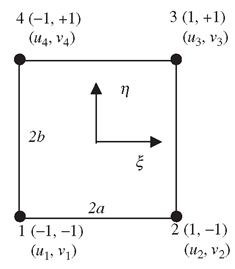
\includegraphics[scale=0.5]{images/square2d.png}
\caption{Generic bilinear quadrilateral element}
\label{fig:4nodes}
\end{figure}
The numerical scheme used and the construction of the amplification matrix for this element can be found in \cite{Geradin}: it follows the same steps as the construction presented in the case of the 2D PML. The resulting amplification matrix has a size of $8\times 8$.
The analysis of the amplification matrix is closely related to the study of the normal modes of deformation of the element. In fact, the eigenvectors of the amplification matrix represent the natural modes and the eigenvalues are the natural frequencies of the deformation associated. For a standard bilinear 4-noded element the natural modes of deformation are represented in the following figure borrowed from \cite{Ling2002}.
\begin{figure}[H]
\centering
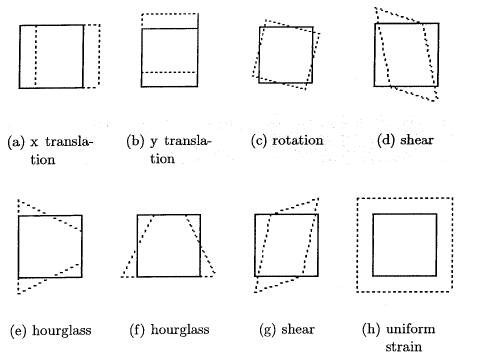
\includegraphics[scale=0.5]{images/def-modes.png}
\caption{Deformation modes corresponding to the eigenmodes on a bilinear quadrilateral element}
\label{fig:def-modes}
\end{figure}
One of these deformation modes is dominant over the other and correspond to $\omega_{max}$ which is the maximum frequency over all the deformation modes. 
According to \cite{Ling2002}, this dominant mode is different in function of the Poisson's ratio. In fact, below a certain transition value the dominant mode is either shear-mode or hourglass mode of deformation depending on the formulation. Above this transition value the uniform normal strain mode dominates. \\
\begin{itemize}
\item \underline{Implicit scheme :} To validate our method let us test it on the Implicit Newmark scheme applied on the discretisation of the equations of motion of the elastic medium. We obtain for several values of time step $h$ taken within the interval $[0.0001, 0.1]$ by steps of $0.0001$. $\omega_{max}$ is taken to be the frequency of the shear mode of deformation. For each value of time step we calculate the amplification matrix and its eigenvalues. We obtain the following representation in the complex plane of the eigenvalues and the spectral radius. For each time step we obtain $8$ eigenvalues since the amplification matrix is of size $8 \times 8$.
\begin{figure}[H]
\centering
\begin{minipage}{.5\textwidth}
  \centering
  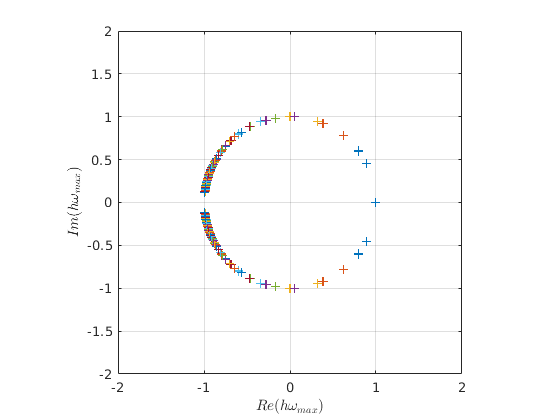
\includegraphics[width=.98\linewidth]{images/eig_med_imp.png}
  \captionof{figure}{Eigenvalues of the amplification matrix in complex plane}
  \label{fig:eig_med_imp}
\end{minipage}%
\begin{minipage}{.5\textwidth}
  \centering
  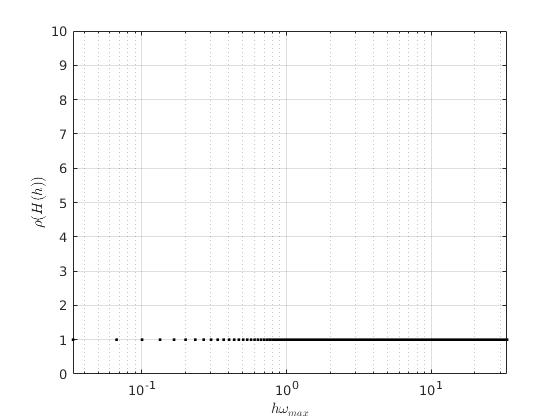
\includegraphics[width=.98\linewidth]{images/spect_rad_med_imp.png}
  \captionof{figure}{Spectral radius of the amplification matrix}
  \label{fig:spect_rad_med_imp}
\end{minipage}
\end{figure}  
As we expected the scheme is stable: this can be observed by looking at the figures \ref{fig:eig_med_imp} and \ref{fig:spect_rad_med_imp}. The representation of the eigenvalues remains in the unit circle and the spectral radius remains below $1$ for all values of the time step.
\begin{figure}[H]
\centering
\begin{minipage}{.5\textwidth}
  \centering
  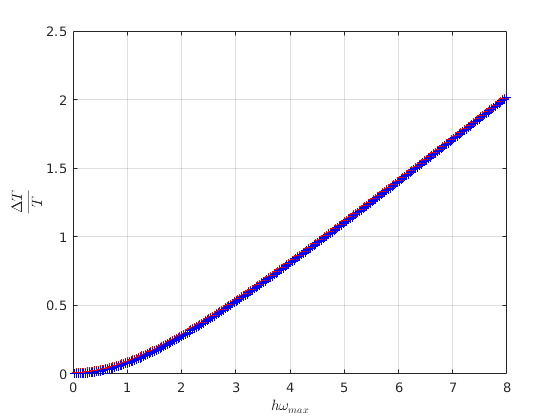
\includegraphics[width=1.\linewidth]{images/per_err_med_imp.png}
  \captionof{figure}{Relative periodicity error}
  \label{fig:per_err_med_imp}
\end{minipage}%
\begin{minipage}{.5\textwidth}
  \centering
  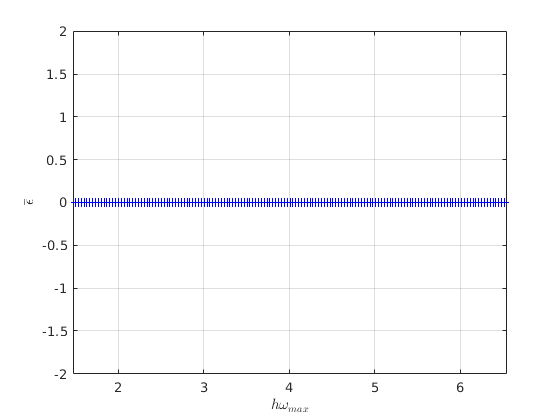
\includegraphics[width=1.\linewidth]{images/num_damp_med_imp.png}
  \captionof{figure}{Numerical damping ratio}
  \label{fig:num_damp_med_imp}
\end{minipage}
\end{figure}   
As we expected the error in term of period increases with the time step (fig. \ref{fig:per_err_med_imp}). The more the time step increases the more the error committed by the scheme is important. The numerical damping ratio remains equal to $0$ because the Newmark implicit scheme is known to not add any artificial damping. 
\item \underline{Explicit Newmark scheme : } The same method with the same values of the time step is used here. We obtained the following results:
\begin{figure}[H]
\centering
\begin{minipage}{.5\textwidth}
  \centering
  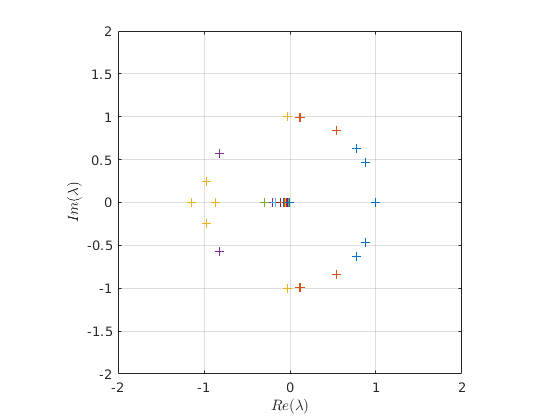
\includegraphics[width=.98\linewidth]{images/eig_med_exp.png}
  \captionof{figure}{Eigenvalues of the amplification matrix in complex plane}
  \label{fig:eig_med_exp}
\end{minipage}%
\begin{minipage}{.5\textwidth}
  \centering
  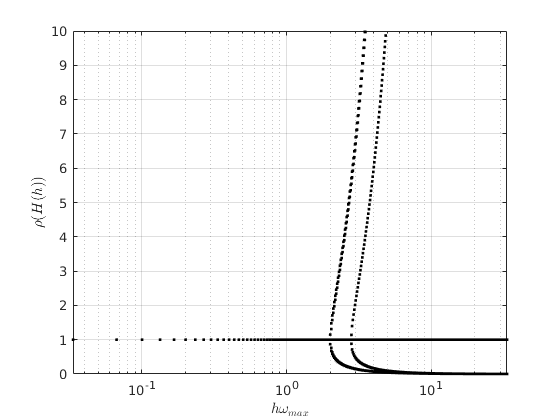
\includegraphics[width=.98\linewidth]{images/spect_rad_med_exp_not_zoom.png}
  \captionof{figure}{Spectral radius of the amplification matrix}
  \label{fig:spect_rad_med_exp_not_zoom}
\end{minipage}
\end{figure} 
The Newmark explicit scheme is known to be conditionally stable, which means that above a certain value of the time step the scheme becomes unstable. This situation appears on the figures \ref{fig:eig_med_exp} where the eigenvalues for a certain time step go out of the unit circle and \ref{fig:spect_rad_med_exp_not_zoom} on which we can observe that the spectral radius of the amplification matrix is above $1$ after a critical value of time step. In the literature \cite{Geradin}, we can find that the critical value is $\omega_{max} h = 2$. Let us make a zoom of the figure \ref{fig:spect_rad_med_exp_not_zoom}:
\begin{figure}[H]
  \centering
  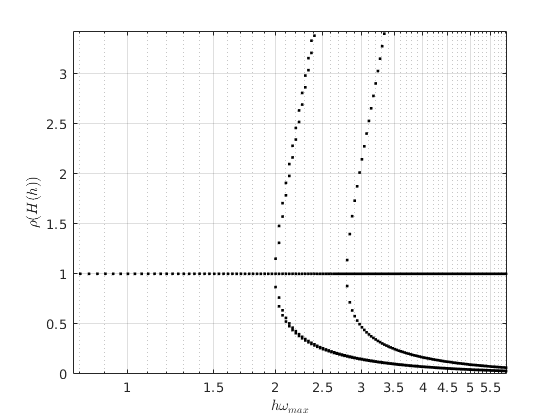
\includegraphics[scale=0.6]{images/spect_rad_med_exp.png}
  \caption{radius of the amplification matrix}
  \label{fig:spect_rad_med_exp}
\end{figure}
We can observe that the scheme becomes unstable for the same value of critical $\omega_{max} h$ than in the literature. \\
Since the integration scheme is unstable, the analysis of the numerical damping ratio and the relative periodicity error is meaningless because their values will be absurd as you can see on the figures \ref{fig:rel_per_err_med_exp} and \ref{fig:num_damp_med_exp}.  
\begin{figure}[H]
\centering
\begin{minipage}{.5\textwidth}
  \centering
  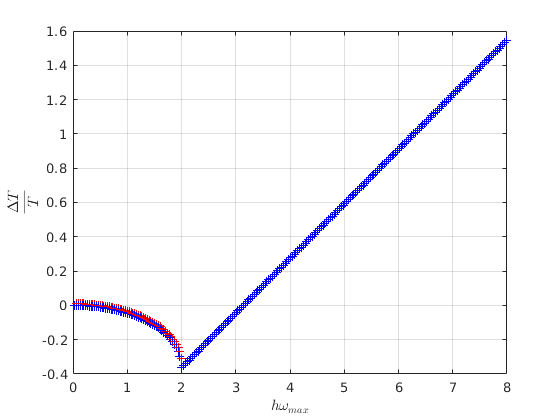
\includegraphics[width=.98\linewidth]{images/rel_per_err_med_exp.png}
  \captionof{figure}{Relative periodicity error}
  \label{fig:rel_per_err_med_exp}
\end{minipage}%
\begin{minipage}{.5\textwidth}
  \centering
  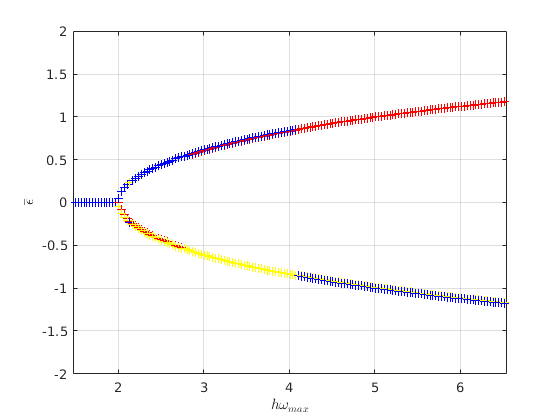
\includegraphics[width=.98\linewidth]{images/num_damp_med_exp.png}
  \captionof{figure}{Numerical damping ratio}
  \label{fig:num_damp_med_exp}
\end{minipage}
\end{figure} 
We can only observe that when the scheme is stable, the relative periodicity error is negative. This result is not surprising since explicit schemes are known to introduce a negative error in terms of period.     
\end{itemize}

\subsubsection{PML element}
Using the previous results we can conclude that our method is able to retrieve the proof of the stability of the Newmark integration scheme associated with the discrete equations of motion of an elastic medium. Let us now review the results obtained with the same integration schemes: Explicit and Implicit Newmark on a PML element.
\begin{itemize}
\item \underline{Implicit Newmark scheme :} Let us calculate the eigenvalues of the amplification matrix associated with the PML for values of the time step $h$ taken in the interval $[1e-3, 1] $ with a step of $1e-3$. The frequency $\omega_{max}$ is taken to be the frequency of the shear mode of deformation of the element without the PML.
The attenuation is supposed to be constant along the element. Therefore, the functions $f_e(x)$ and $f_p(x)$ are equal to $10$ and are constant along the element.
On the two following figures, we will represent all the eigenvalues in the complex plane and their modulus for each time step. 
\begin{figure}[H]
\centering
\begin{minipage}{.5\textwidth}
  \centering
  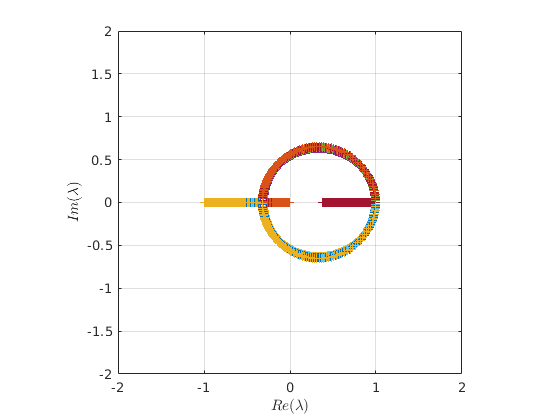
\includegraphics[width=1.\linewidth]{images/eig_pml_imp_10.png}
  \captionof{figure}{eigenvalues in the complex plane}
  \label{fig:eig_pml_imp_10}
\end{minipage}%
\begin{minipage}{.5\textwidth}
  \centering
  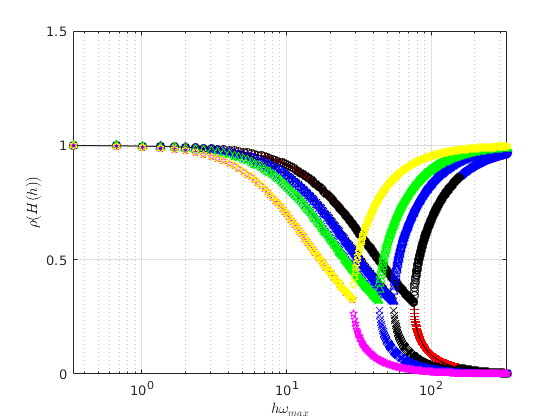
\includegraphics[width=1.\linewidth]{images/spect_rad_pml_imp_10.png}
  \captionof{figure}{Moduli of the eigenvalues}
  \label{fig:spect_rad_pml_imp_10}
\end{minipage}
\end{figure} 
By analizing the two figures \ref{fig:eig_pml_imp_10} and \ref{fig:spect_rad_pml_imp_10}, we can observe that the implicit scheme associated with the pml is unconditionally stable since the eigenvalues remain in the unit circle. They are not precisely on it because the attenuation in the element decreases the amplitude of the deformation. As we can see on the figure \ref{fig:spect_rad_pml_imp_10} the moduli of the eigenvalues decrease and this decay starts at a certain frequency.\\
By increasing the attenuation in the element, another property of the PML can be shown. Let us consider $f_p = f_e = 100$ and reproduce the same figures. 
\begin{figure}[H]
\centering
\begin{minipage}{.5\textwidth}
  \centering
  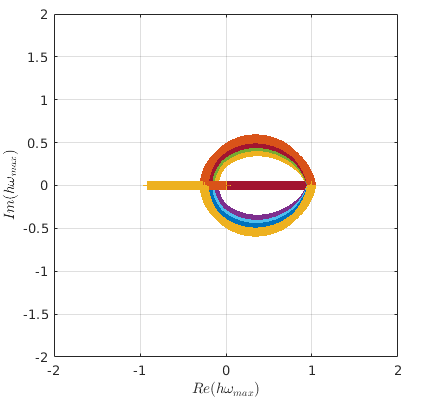
\includegraphics[width=1.\linewidth]{images/eig_pml_imp_100.png}
  \captionof{figure}{eigenvalues in the complex plane}
  \label{fig:eig_pml_imp_100}
\end{minipage}%
\begin{minipage}{.5\textwidth}
  \centering
  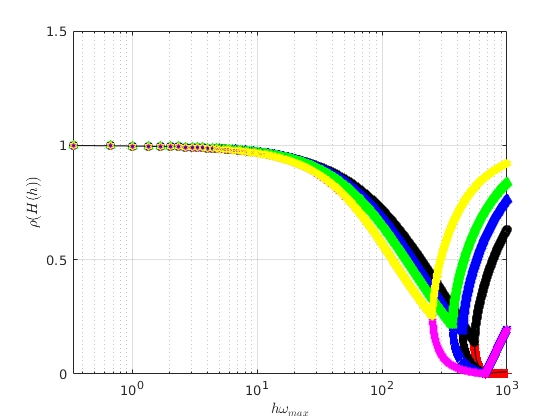
\includegraphics[width=1.\linewidth]{images/spect_rad_pml_imp_100.png}
  \captionof{figure}{Moduli of the eigenvalues}
  \label{fig:spect_rad_pml_imp_100}
\end{minipage}
\end{figure} 
Comparing the figures \ref{fig:eig_pml_imp_10} and \ref{fig:eig_pml_imp_100}, we can observe that the circles formed by the representation of the eigenvalues is flatter when the attenuation is stronger. We can conclude that the attenuation of all modes of deformation is stronger when we increase the attenuation. By comparing the figures \ref{fig:spect_rad_pml_imp_10} and \ref{fig:spect_rad_pml_imp_100} we can observe that the range of frequencies attenuated by the PML becomes larger when we increase the attenuation. This result highlights a property of the PML: we can attenuate waves of all frequencies by a careful choice of the parameter of the PML. Also, we can observe that choosing a higher value of attenuation leads to the ability of the PML to attenuate higher frequencies. \\
Let us now review the results concerning the relative periodicity error and the numerical damping ratio. We pick again the value of attenuation $f_p = f_e = 10$. An important observation with the formulation of the amplification matrix is that it leads to the calculation of eigenvalues and eigenmodes of deformation not related to any "physical" mode of deformation. This is of course due to the fact that the PML is not a physical material, its only purpose is to attenuate wave and this leads to the presence of spurious modes. Their values of relative periodicity error and numerical damping ratio are not to be considered and are in fact aberrant. The main thing that we already reviewed is, for the implicit scheme, they do not lead to the instability of the scheme. We will consider in this part, the analysis of the results for the dominant mode of deformation, the shear mode.  
\begin{figure}[H]
\centering
\begin{minipage}{.5\textwidth}
  \centering
  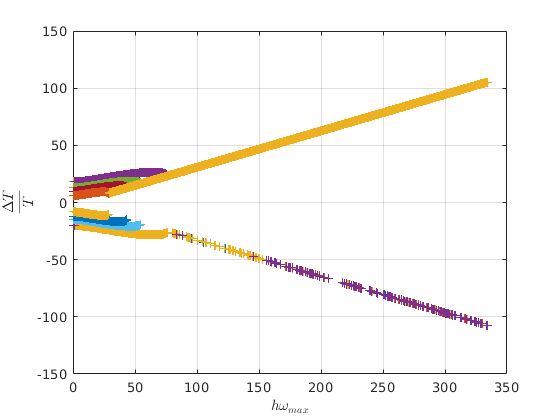
\includegraphics[width=1.\linewidth]{images/rel_per_err_pml_imp_10.png}
\end{minipage}%
\begin{minipage}{.5\textwidth}
  \centering
  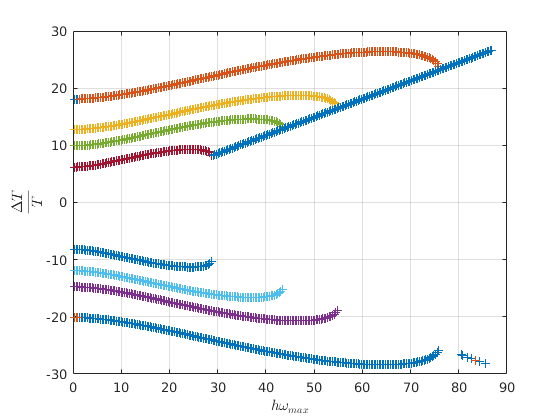
\includegraphics[width=1.\linewidth]{images/rel_per_err_pml_imp_10_80.png}
\end{minipage}%
\captionof{figure}{Relative periodicity error}
\label{fig:rel_per_err_pml_imp_10}
\end{figure}

\begin{figure}[H]
\centering
\begin{minipage}{.5\textwidth}
  \centering
  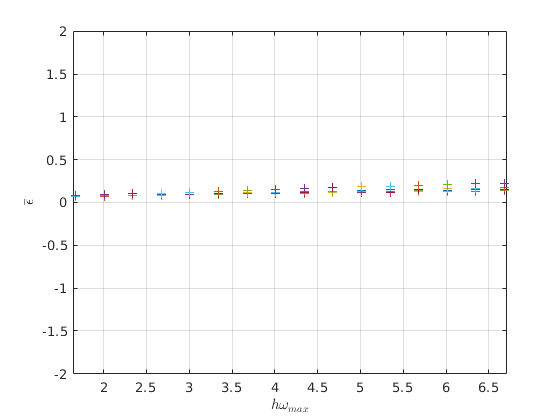
\includegraphics[width=1.\linewidth]{images/num_damp_pml_imp_10.png}
\end{minipage}%
\begin{minipage}{.5\textwidth}
  \centering
  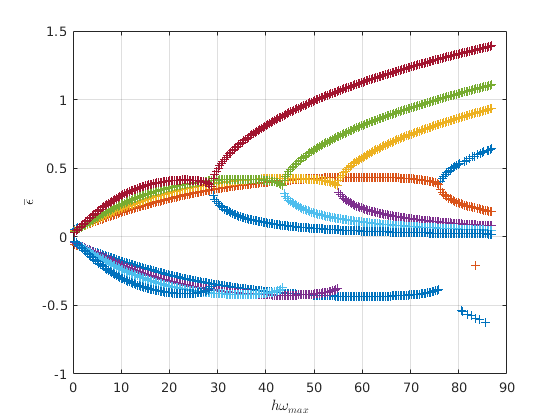
\includegraphics[width=1.\linewidth]{images/num_damp_pml_imp_10_80.png}
\end{minipage}
\captionof{figure}{Numerical damping ratio}
\label{fig:num_damp_pml_imp_10}
\end{figure} 
It is difficult to analyse precisely the results of the relative periodicity error shown on the figure \ref{fig:rel_per_err_pml_imp_10}. The PML is not a physical medium and the error in period is not important since its purpose is to attenuate the wave and not propagating it. Therefore the error in period is not too important and it increases with larger values of the time step which is a common result for numerical simulation schemes. The PML is conceived to introduce an artificial damping in the system, this is why we can observe on the figure \ref{fig:num_damp_pml_imp_10} that, even the implicit Newmark scheme associated with the PML introduce a numerical damping. This attenuation increases with the frequency of the wave. Of course by increasing the attenuation in the element the numerical damping ratio will take bigger values.
\item \underline{Explicit Newmark scheme :}
We have shown in the previous part concerning the standard element stability analysis that the Explicit scheme is conditionally stable and the critical value  $\omega h = 2$. Therefore, for the stability analysis of the same scheme associated with the PML we will dedicate a specific attention to the critical value where the scheme starts to become unstable. 
For $f_p = f_e = 10$, we obtain the following results:
\begin{figure}[H]
\centering
\begin{minipage}{.5\textwidth}
  \centering
  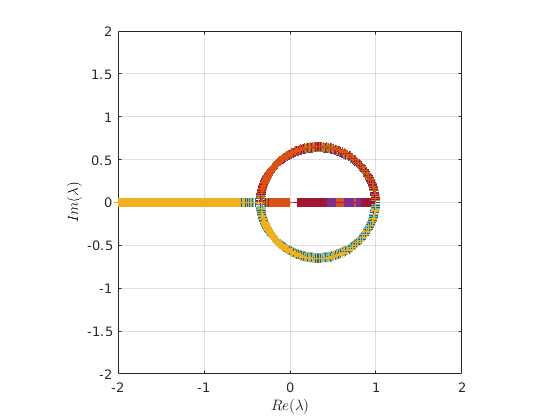
\includegraphics[width=.99\linewidth]{images/eig_pml_exp_10.png}
  \captionof{figure}{Eigenvalues of the amplification matrix in complex plane}
  \label{fig:eig_pml_exp_10}
\end{minipage}%
\begin{minipage}{.5\textwidth}
  \centering
  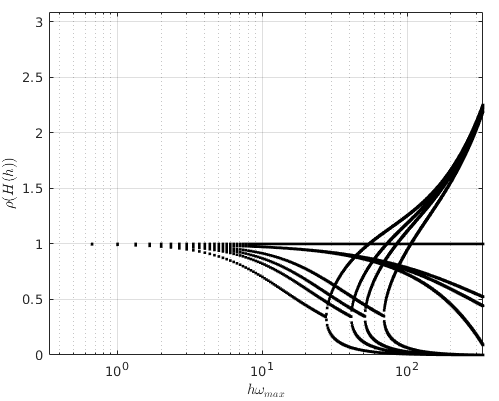
\includegraphics[width=.99\linewidth]{images/spect_rad_pml_exp_10.png}
  \captionof{figure}{Spectral radius}
  \label{fig:spect_rad_pml_exp_10}
\end{minipage}
\end{figure} 
The stability of the explicit scheme associated with the PML is also conditionally stable because, as we can observe on the figure \ref{fig:eig_pml_exp_10}, the representation of the eigenvalues in the complex plane goes out the unit circle from a certain value of $\omega_{max} h$. Looking at the figure \ref{fig:spect_rad_pml_exp_10}, we can determine this limit of stability. We can find that the critical value is $\omega_{max} h = 80$ which is of course larger than the limit of the stability of the explicit scheme associated with the standard element. Therefore we can ask ourselves why the limit of stability is extended. Some features of the PML must impact the scheme in this manner. Let us focus on the attenuation and increase the value to $f_p = f_e = 100$.
\begin{figure}[H]
\centering
\begin{minipage}{.5\textwidth}
  \centering
  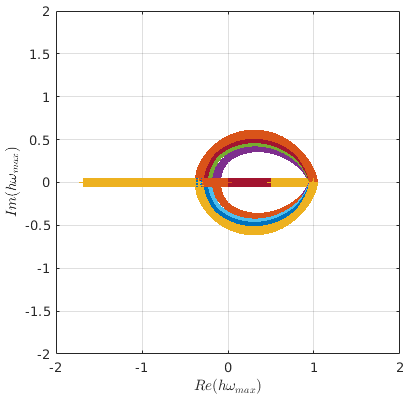
\includegraphics[width=.90\linewidth]{images/eig_pml_exp_100.png}
  \captionof{figure}{Eigenvalues of the amplification matrix in complex plane}
  \label{fig:eig_pml_exp_100}
\end{minipage}%
\begin{minipage}{.5\textwidth}
  \centering
  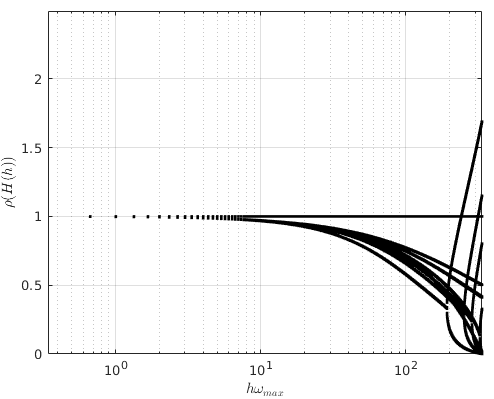
\includegraphics[width=.99\linewidth]{images/spect_rad_pml_exp_100.png}
  \captionof{figure}{Spectral radius}
  \label{fig:spect_rad_pml_exp_100}
\end{minipage}
\end{figure} 
The first observation that can be made using the figure \ref{fig:eig_pml_exp_100} is the same as in the context of the implicit scheme: increasing the attenuation makes the representation of the circle formed by the eigenvalues flatter. This is due to the fact that the amplitude of the deformation is attenuated in a stronger manner when the attenuation coefficient is larger. Secondly, using the figure \ref{fig:spect_rad_pml_exp_100}, we can observe that by increasing the attenuation the critical value where the scheme becomes unstable is postponed to $\omega_{max} h = 200$. We can conclude that the attenuation impacts the explicit scheme and permits to take larger value of the time step while keeping the stability. An hypothesis to explain this observation is that the attenuation affects the amplitude of the deformation and therefore, is able to decay a finite variation of the state vector. This results in postponing the critical value of the time step for which this finite variation becomes too large to not introduce a non-increasing variation of the state vector at a subsequent time. \\
Since the scheme becomes unstable at a certain value of time step the analysis of the relative periodicity error and of the numerical damping ratio is difficult. Let us review the result using only the shear mode of deformation since it is the dominant one. We will look at the results obtained when the scheme remains stable $h < h_{crit}$. After this value the results can not be analysed since the values become too large.  
\begin{figure}[H]
\centering
\begin{minipage}{.5\textwidth}
  \centering
  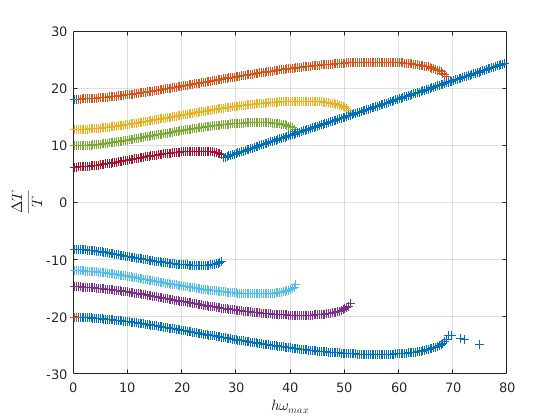
\includegraphics[width=.90\linewidth]{images/rel_per_err_pml_exp_10.png}
  \captionof{figure}{Relative periodicity error}
  \label{fig:rel_per_err_pml_exp_10}
\end{minipage}%
\begin{minipage}{.5\textwidth}
  \centering
  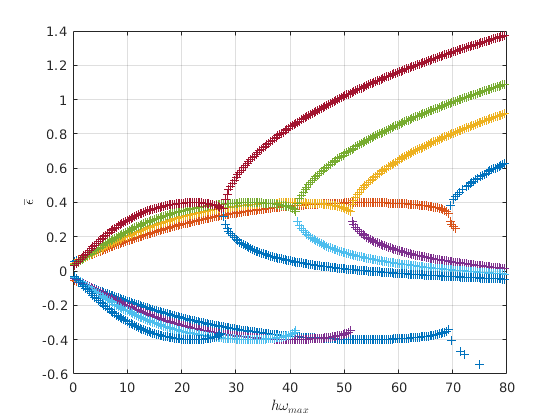
\includegraphics[width=.99\linewidth]{images/num_damp_pml_exp_10.png}
  \captionof{figure}{Numerical damping ratio}
  \label{fig:num_damp_pml_exp_10}
\end{minipage}
\end{figure}   
Comparing to the figures \ref{fig:rel_per_err_pml_imp_10} and \ref{fig:num_damp_pml_imp_10} the results obtained in the stable part of the explicit scheme follows the same trends. Therefore the same observation can be made. The periodicity error, shown on the figure \ref{fig:rel_per_err_pml_exp_10} is difficult to analyse. We can observe that the conjugated eigenvalues separate: one shows a positive periodicity error and the other one a negative. We can also clearly distinguish the 2 shear modes of deformation and the 2 hourglass modes. As the time step increases, they seem to meet in the same linear curve. After this joining we can not observe separately the eigenvalues correpsonding to different shear and hourglass modes. A close observation can be made about the numerical damping ratio using the figure \ref{fig:num_damp_pml_exp_10}. Here the numerical damping ratios obtained using the different eigenvalues associated with shear and hourglass modes do not seem to converge to a common curve. In fact at the beginning we can clearly identify the 2 shear modes and the 2 hourglass modes of deformation. The numerical damping ratio is positive and it corresponds to the attenuation present in the element. At a certain value of time step (different for each shear and hourglass mode of deformation), a separation can be observed for the numerical damping ratio associated with conjugated eigenvalues. The lower branches tend to $0$ whereas the upper ones do not seem to converge to a certain value. The slope of the evolution of numerical damping for the upper branches seems to become weaker as the time step increases.      
\end{itemize} 
